\chapter{OFDM in 4G-LTE Mobile Networks}

\indent 4G-LTE (\textit{4th Generation-Long Term Evolution}, or \textit{3GPP-LTE}, here designated as LTE) is the commercial name of a standard for a communication protocol (physical layer), developed by the 3GPP (\textit{3rd Generation Partnership Project}) and released progressively in different countries around the world, since first launch in Stockholm and Oslo in 2009.

\section{4G-LTE Overview}
%
\indent LTE has been designed as an evolution to former mobile communication techniques (GSM, UMTS, CDMA2000) `to increase 
data rates, improve spectrum efficiency, improve coverage, and reduce latency'\cite{EDahlman}. 4G-LTE was not actually intended to be a proper 4th Generation technology by the 3GPP consortium. However, the initial goal of this \textit{Long Term Evolution} technology is to ensure that 3G can stay competitive throughout years.\\
\indent For instance, one of its definition items actually states that it should reach a \si{100\ Mbps} for the downlink and \si{50\ Mbps} for the uplink and can therefore be used both for voice and data. The difference between the uplink and downlink can be explained with the fact that two slightly different technologies are used.

\section{LTE Technical Considerations}
%
\indent Since, mobile communications usually operate between a BS and a MS (\textit{Mobile Station}), the LTE standard defines rules that accounts for the constraints and advantages of both sides. While, BS don't face the issues from high power-consumption, MS for instance, need a communication technology that doesn't drain all their available power.\\
%
\indent Thus, OFDMA communication technique, described in \secref{sec:OFDMA}, is used as is on the BS side, which allows for \textit{Muliple Access}, to respond a network cell's needs in high traffic and convenient data rates.\\
%
\indent These throughputs can be achieved by chosing the right symbol rate, which is directly influenced by the frequency separation between each subcarrier and therefore, by the number of subcarriers in a channel. Different channel bandwidths are defined in LTE\cite{RadioElLTE}:
\begin{itemize}
  \setlength\itemsep{0.2em}
  \item  1.4 MHz
  \item  3 MHz
  \item  5 MHz
  \item  10 MHz
  \item  15 MHz
  \item  20 MHz.
\end{itemize}
\indent Meanwhile, the sub-carrier spacing, $\Delta f$, is set to \si{15\ kHz}, which yields \si{15\ ksps} and a symbol time of:
\begin{flalign}
\eq{T_S}{\frac{1}{15 \cdot 10^3}}&\nonumber\\
\eq{T_S}{66,7 \cdot 10^{-6}}\si{s}&\nonumber \\
\eq{T_S}{66,7}\si{\mu s}.&\nonumber
\end{flalign}\\ 
\indent Eventually, using a \si{20\ MHz} channel bandwidth (which allows for 100 frequency resource blocks of 12 subcarriers) and a 64QAM (which means 6 bits are used to map bits of data in one symbol), results in having a theoretical data rate of \si{108\ Mbps}. However, the signal being affected by several physical and environmental factors, the real data rate is actually lower.\\
\indent Moreover, the cycling prefix, $T_{CP}$, used by OFDM to reduce ISI even more than allowed by the low symbol time, is defined for LTE as :
\begin{flalign}
\eq{T_{CP}}{4,69}\si{\mu s}.&\nonumber
\end{flalign}\\ 
%
\indent While simple OFDMA happens at BS side, and the previously defined standards remain the same, the technique used on the MS side is slightly modified into what is called SC-FDMA (\textit{Single Carrier - Frequency Division Multiple Access}), which allows to lower the peak-to-average ratio and thus, reduce the power consumption over time. This is achieved by having the users (MS) to apply a supplementary DFT before bit mapping (compensated on the receiver end by an IDFT after de-mapping) and use a single-carrier structure, see \figref{fig:SCFDMAGenerator}.
%
\begin{figure}[H]
  \centering
  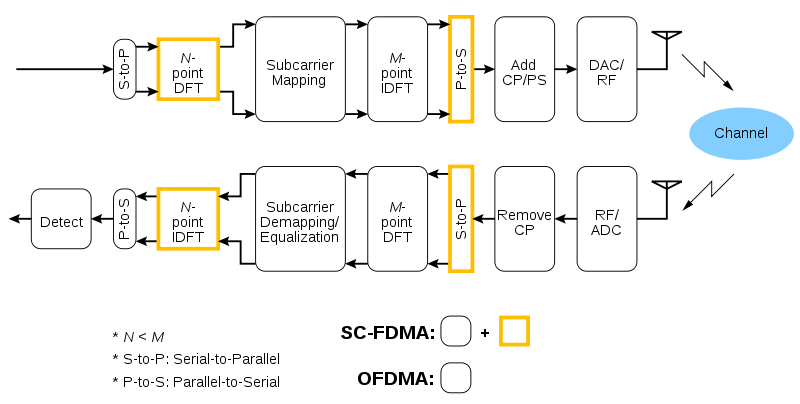
\includegraphics[width=\textwidth]{figures/SC-FDMA.png}
  \caption{SC-FDMA signal generation\textbf{[source: Wikipedia]}}
  \label{fig:SCFDMAGenerator}
\end{figure}